\documentclass[10pt]{beamer}
\usepackage[utf8]{inputenc}

\usetheme{metropolis}

\usepackage{acronym} % \ac[p], \acl[p], \acs[p], \acf[p]
\usepackage{appendixnumberbeamer}
\usepackage[scale=2]{ccicons}
\usepackage[absolute, overlay]{textpos}
\usepackage{tikz}
\usetikzlibrary{positioning}
\usepackage{transparent}

% Acronyms
% --------
\acrodef{CRDT}[CRDT]{Conflict-free Replicated Data Type}
\acrodefplural{CRDT}[CRDTs]{Conflict-free Replicated Data Types}

\author{
  Matthieu Nicolas
  \\
  COAST team
  \\
  \textbf{Supervised by} Gérald Oster and Olivier Perrin
}
\title{Efficient renaming in \acp{CRDT}}
\institute{
  \vspace{3em}
  
\includegraphics[width=2.8cm]{img/loria-logo.png}\hspace{3em}
  
\includegraphics[width=1.2cm]{img/ul-logo.pdf}\hspace{3em}
  
\includegraphics[width=3cm]{img/inria-logo.pdf}\hspace{3em}
  
\includegraphics[width=1.2cm]{img/cnrs-logo.png}
}

\setbeamertemplate{bibliography item}[text]

\begin{document}

\begin{frame}[t,plain]
  \maketitle
\end{frame}

\begin{frame}{\acfp{CRDT} \cite{shapiro_2011_crdt}}
  \begin{columns}
    \begin{column}{0.65\textwidth}
      \begin{tikzpicture}

        \node (A) at (0, 0) {
\includegraphics{img/blue-node.pdf}};
        \node[below=3pt of A] {\textbf{A}};
        \node<1>[above=3pt of A] {
\includegraphics[scale=0.6]{img/doc.pdf}};
        \node<2-4>[above=3pt of A] {
\includegraphics[scale=0.6]{img/docA.pdf}};
        \node<5->[above=3pt of A] {
\includegraphics[scale=0.6]{img/docABC.pdf}};

        \node (B) at (-2, -3) {
\includegraphics{img/red-node.pdf}};
        \node[below=3pt of B] {\textbf{B}};
        \node<1-2>[left=3pt of B] {
\includegraphics[scale=0.6]{img/doc.pdf}};
        \node<3>[left=3pt of B] {
\includegraphics[scale=0.6]{img/docA.pdf}};
        \node<4>[left=3pt of B] {
\includegraphics[scale=0.6]{img/docAB.pdf}};
        \node<5->[left=3pt of B] {
\includegraphics[scale=0.6]{img/docABC.pdf}};

        \transparent{0.2}
          \node<-4> (C) at (2, -3) {
\includegraphics{img/green-node.pdf}};
          \node<1-3>[right=3pt of C] {
\includegraphics[scale=0.6]{img/doc.pdf}};
        \transparent{1}
        \node<4-> at (2, -3) {
\includegraphics{img/green-node.pdf}};
        \node<4>[right=3pt of C] {
\includegraphics[scale=0.6]{img/docC.pdf}};
        \node[below=3pt of C] {\textbf{C}};
        \node<5->[right=3pt of C] {
\includegraphics[scale=0.6]{img/docABC.pdf}};

        \draw[shorten >=3pt, shorten <=3pt]
          (A) to[bend right] (B)
          (B) to[bend right] (C)
          (C) to[bend right] (A);

        \node<2>[below left=-30pt and 5pt of A] {
\includegraphics[scale=0.4]{img/blue-update.pdf}};
        \node<2, 4>[below right=-30pt and 5pt of A] {
\includegraphics[scale=0.4]{img/blue-update.pdf}};

        \node<4>[below right=-4pt and 1pt of B] {
\includegraphics[scale=0.6]{img/red-update.pdf}};
        \node<4>[above left=1pt and -15pt of B] {
\includegraphics[scale=0.6]{img/red-update.pdf}};

        \node<4>[below left=-4pt and 1pt of C] {
\includegraphics[scale=0.6]{img/green-update.pdf}};
        \node<4>[above right=1pt and -15pt of C] {
\includegraphics[scale=0.6]{img/green-update.pdf}};
      \end{tikzpicture}
    \end{column}
    \begin{column}{0.35\textwidth}
      \begin{itemize}
        \item Replicated data structure
        \item<2-> Updates performed without coordination
        \item<5-> Strong Eventual Consistency \cite{shapiro_2011_crdt}
      \end{itemize}
    \end{column}
  \end{columns}
\end{frame}

% \begin{frame}{Large-scale system}
%   \begin{center}
%     \begin{tikzpicture}
%       \node (A) {
\includegraphics{img/blue-node.pdf}};
%       \node[below left=0.5 and -0.2 of A] (B) {
\includegraphics{img/red-node.pdf}};
%       \node[below right=0.5 and -0.2 of A] (C) {
\includegraphics{img/green-node.pdf}};

%       \node[above left=0.5 and -0.2 of B] (D) {
\includegraphics{img/black-node.pdf}};
%       \transparent{0.2}\node[below left=0.5 and -0.2 of D] (E) {
\includegraphics{img/black-node.pdf}};
%       \transparent{1}\node[above left=0.5 and -0.2 of D] (H) {
\includegraphics{img/black-node.pdf}};
%       \node[above right=0.5 and -0.2 of D] (I) {
\includegraphics{img/black-node.pdf}};

%       \transparent{0.2}\node[above right=0.5 and -0.2 of C] (F) {
\includegraphics{img/black-node.pdf}};
%       \transparent{1}\node[below right=0.5 and -0.2 of F] (G) {
\includegraphics{img/black-node.pdf}};
%       \node[above right=0.5 and -0.2 of F] (J) {
\includegraphics{img/black-node.pdf}};
%       \node[above left=0.5 and -0.2 of F] (K) {
\includegraphics{img/black-node.pdf}};

%       \node[below left=0.5 and -0.2 of B] (M) {
\includegraphics{img/black-node.pdf}};
%       \node[below right=0.5 and -0.2 of C] (N) {
\includegraphics{img/black-node.pdf}};

%       \node[left=of E] (O) {};
%       \node[left=of H] (P) {};

%       \node[right=of G] (Q) {};
%       \node[right=of J] (R) {};

%       \draw
%       (A) -- (B)
%       (B) -- (C)
%       (C) -- (A)

%       (B) -- (D)
%       (D) -- (E)
%       (E) -- (M)
%       (B) -- (M)

%       (A) -- (I)
%       (I) -- (D)
%       (D) -- (H)

%       (C) -- (F)
%       (F) -- (G)
%       (G) -- (N)
%       (N) -- (C)

%       (A) -- (K)
%       (K) -- (F)
%       (F) -- (J)

%       (E) -- (O)
%       (H) -- (P)
%       (G) -- (Q)
%       (J) -- (R);
%     \end{tikzpicture}
%   \end{center}
% \end{frame}

\begin{frame}{Identifier-based \acp{CRDT}}
  \begin{block}{Main idea}
    \begin{itemize}
      \item Attach an identifier to each inserted element
    \end{itemize}
  \end{block}

  \bigskip

  % TODO: Rework this block, not sure of what i was saying back then
  \begin{block}{Allow to achieve commutative updates}
    \begin{itemize}
      \item By identifying uniquely elements
      \item By ordering them relatively to each other
    \end{itemize}
  \end{block}
\end{frame}

\begin{frame}{LogootSplit \cite{AndreCollaborateCom2013}}
  \begin{itemize}
    \item State of the art of \emph{Sequence \acp{CRDT}}
    \item Relies on \emph{identifiers} to ensure convergence, noted here as letters and words
    \item Elements are ordered by their identifier
  \end{itemize}

  \pause

  \begin{columns}
    \begin{column}{0.5\textwidth}
      \begin{figure}
        
\includegraphics[scale=0.15]{img/helo-as-letters.png}
        \caption{The state of a sequence which contains the elements "helo" and their corresponding identifiers}
      \end{figure}
    \end{column}
    \pause
    \begin{column}{0.5\textwidth}
      \begin{figure}
        
\includegraphics[scale=0.15]{img/helo-as-block.png}
        \caption{The state of a sequence which contains the block "helo"}
      \end{figure}
    \end{column}
  \end{columns}
\end{frame}

\begin{frame}{Example}
  \begin{figure}
    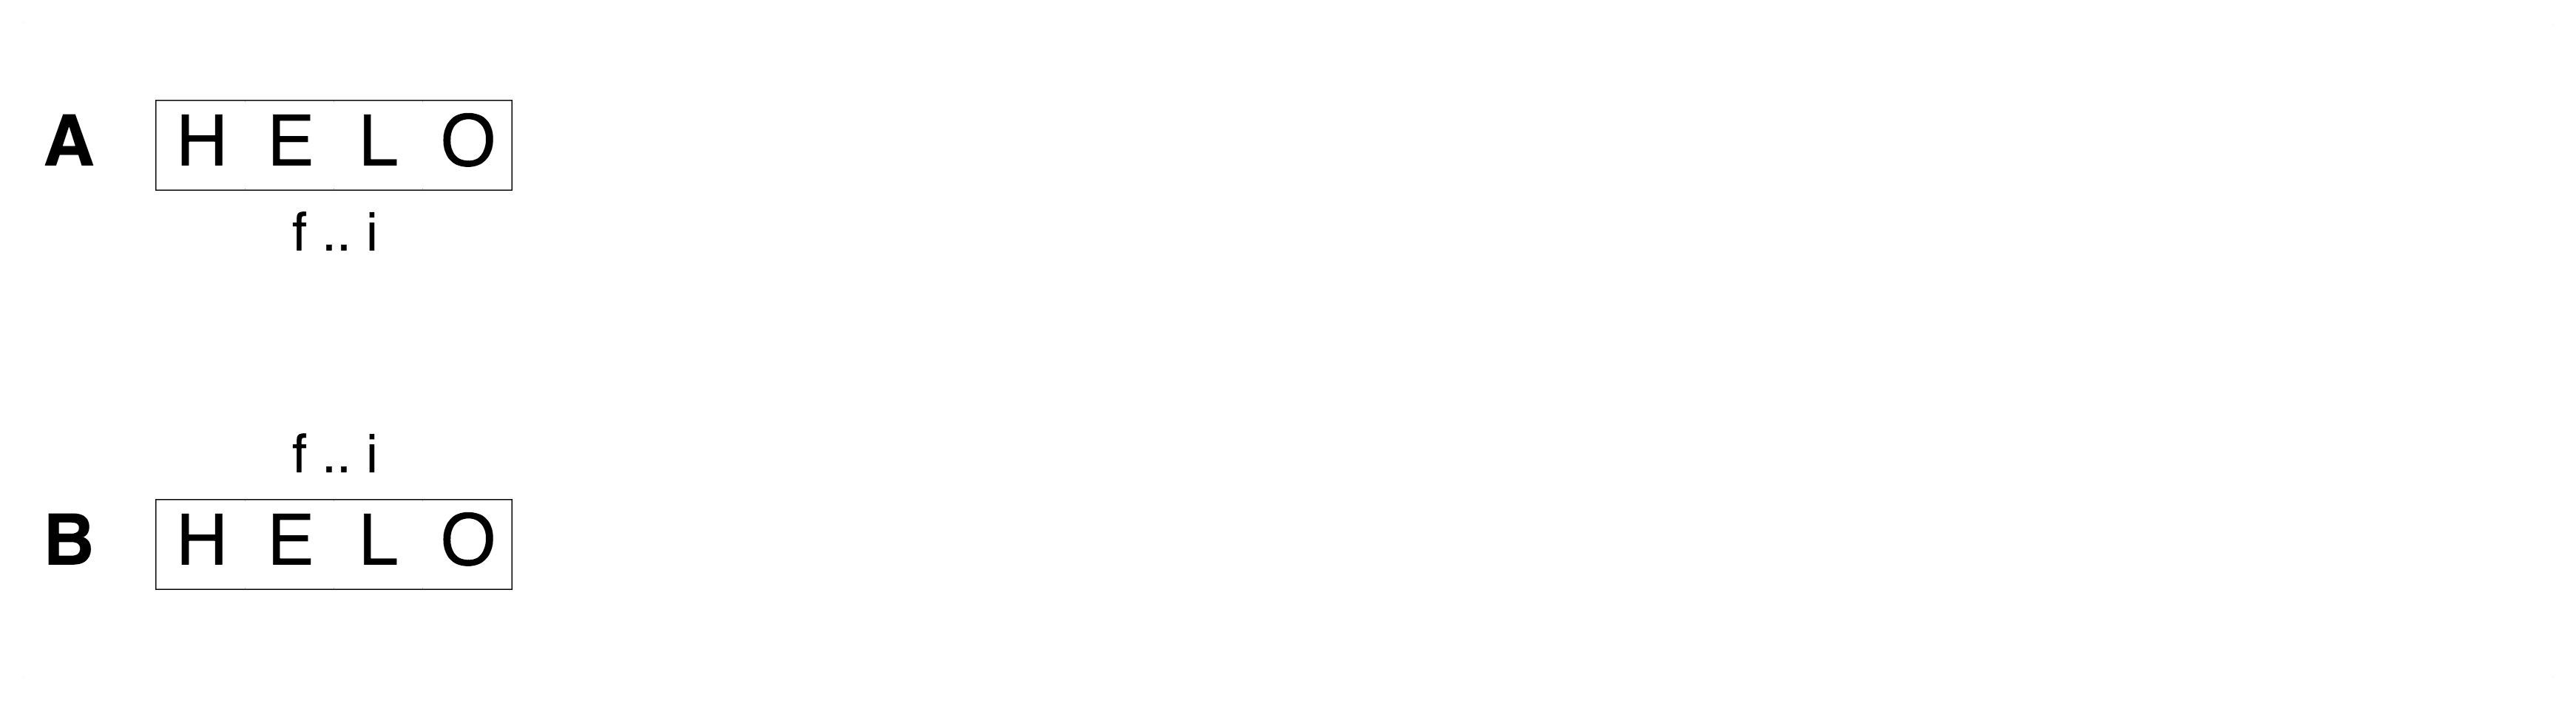
\includegraphics[scale=0.09]{img/initial-state.png}<1-1>
    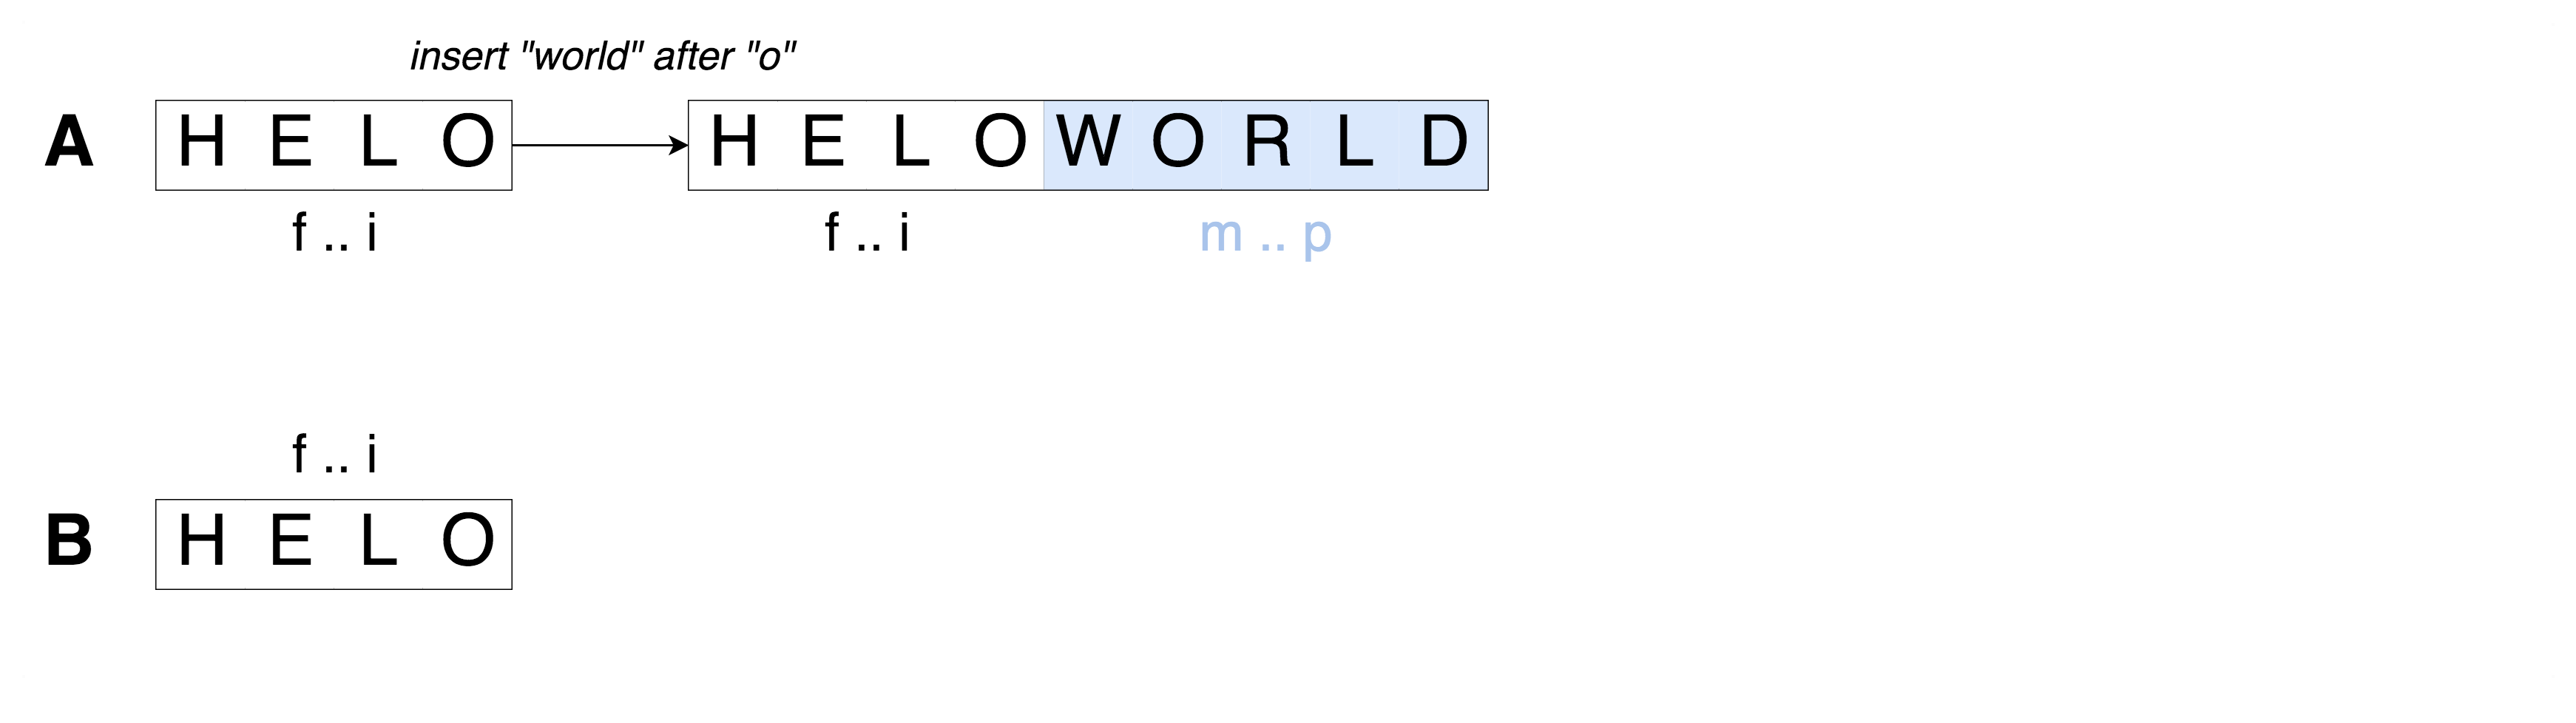
\includegraphics[scale=0.09]{img/insert-world.png}<2-2>
    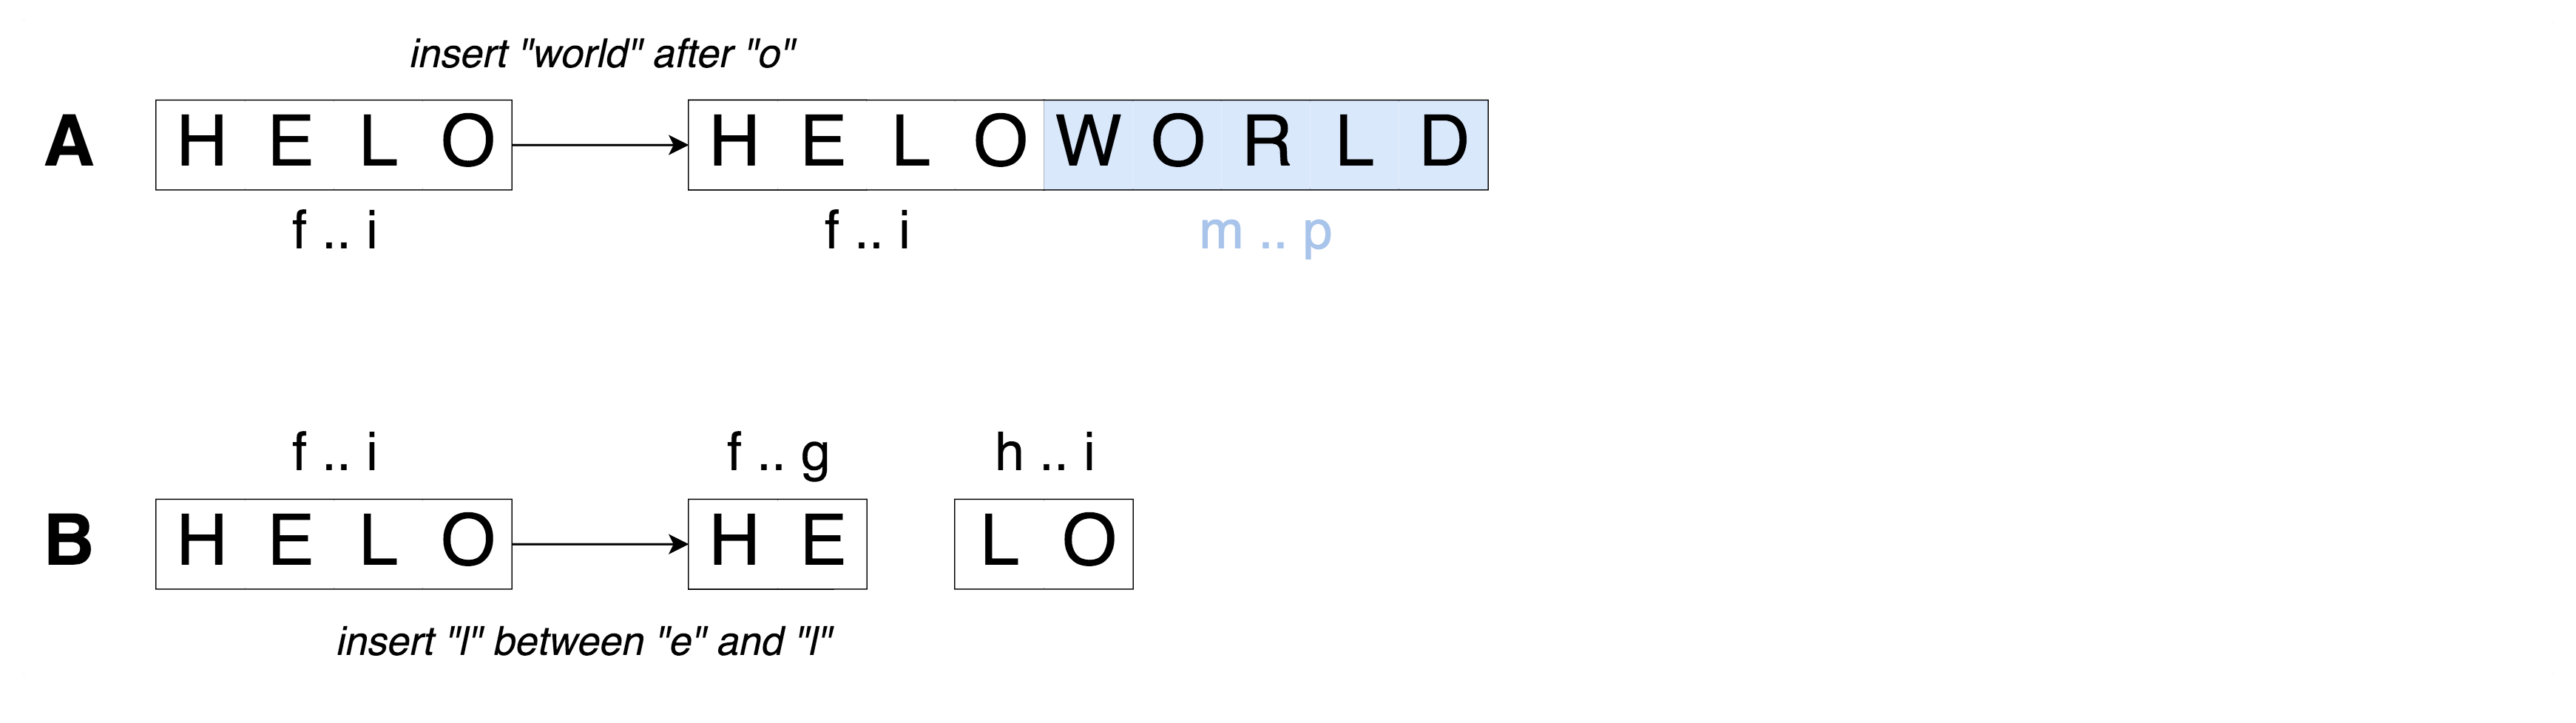
\includegraphics[scale=0.09]{img/insert-split.png}<3-3>
    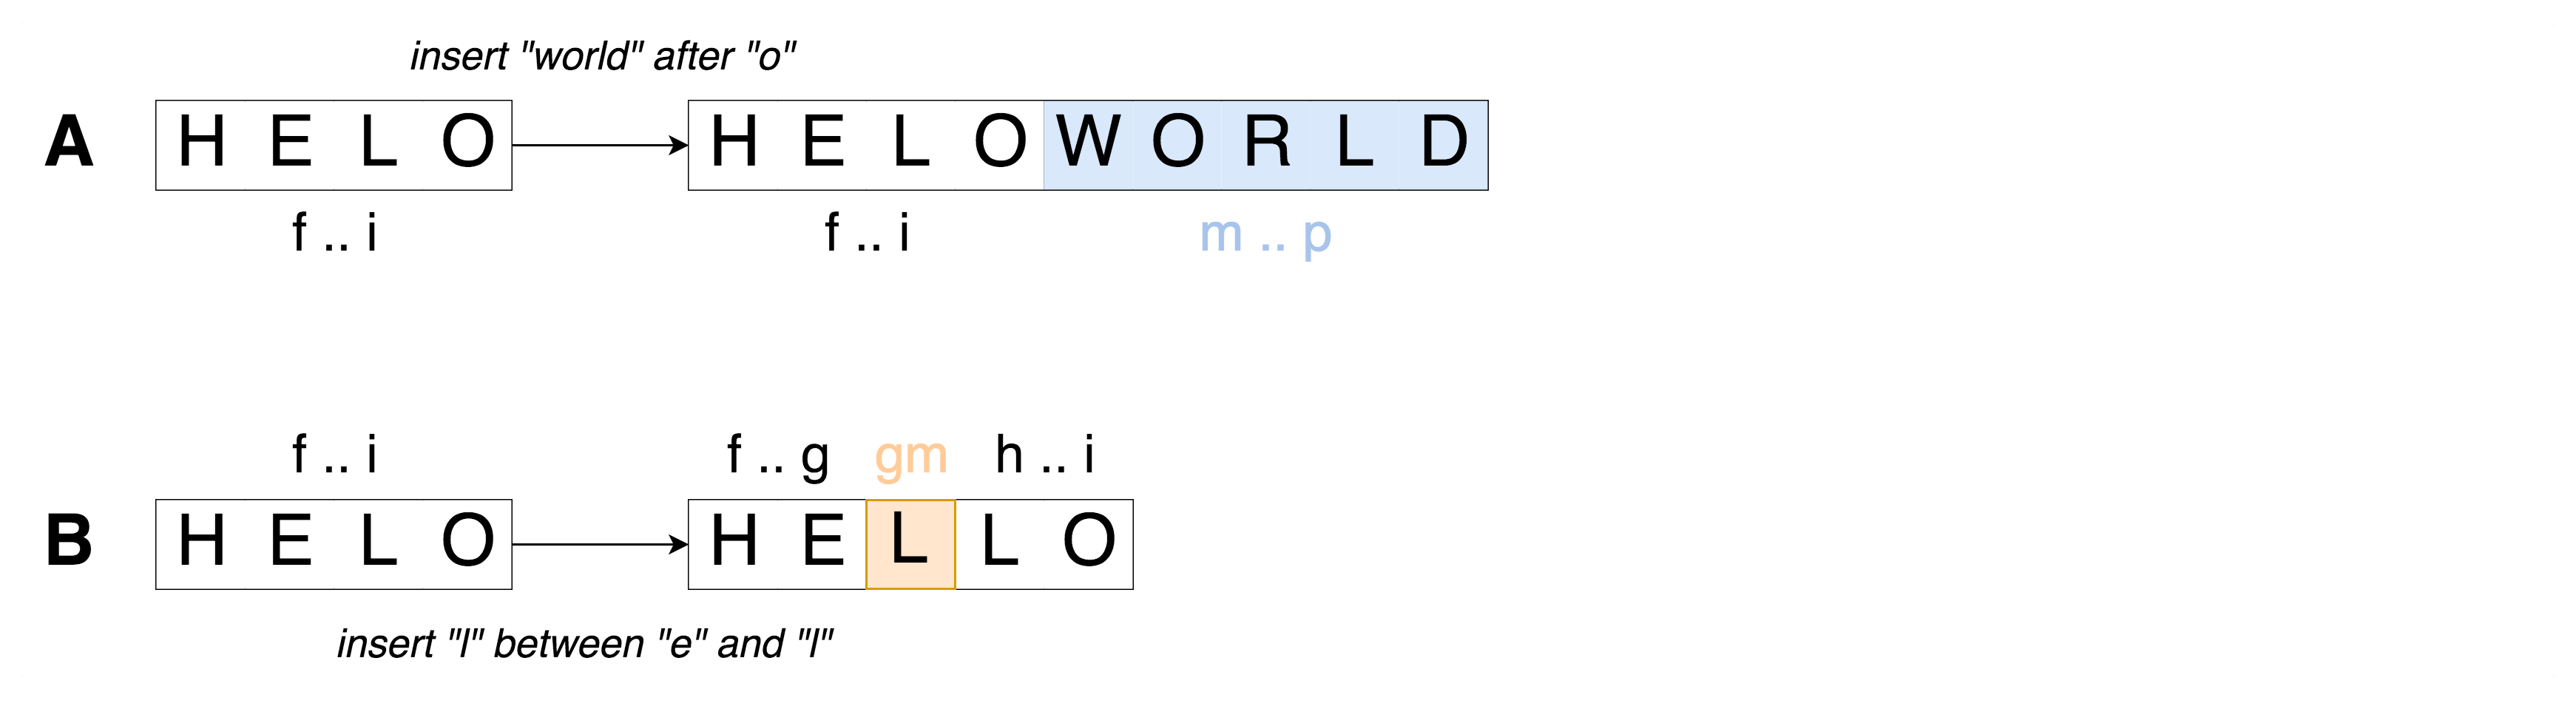
\includegraphics[scale=0.09]{img/insert-l.png}<4-4>
    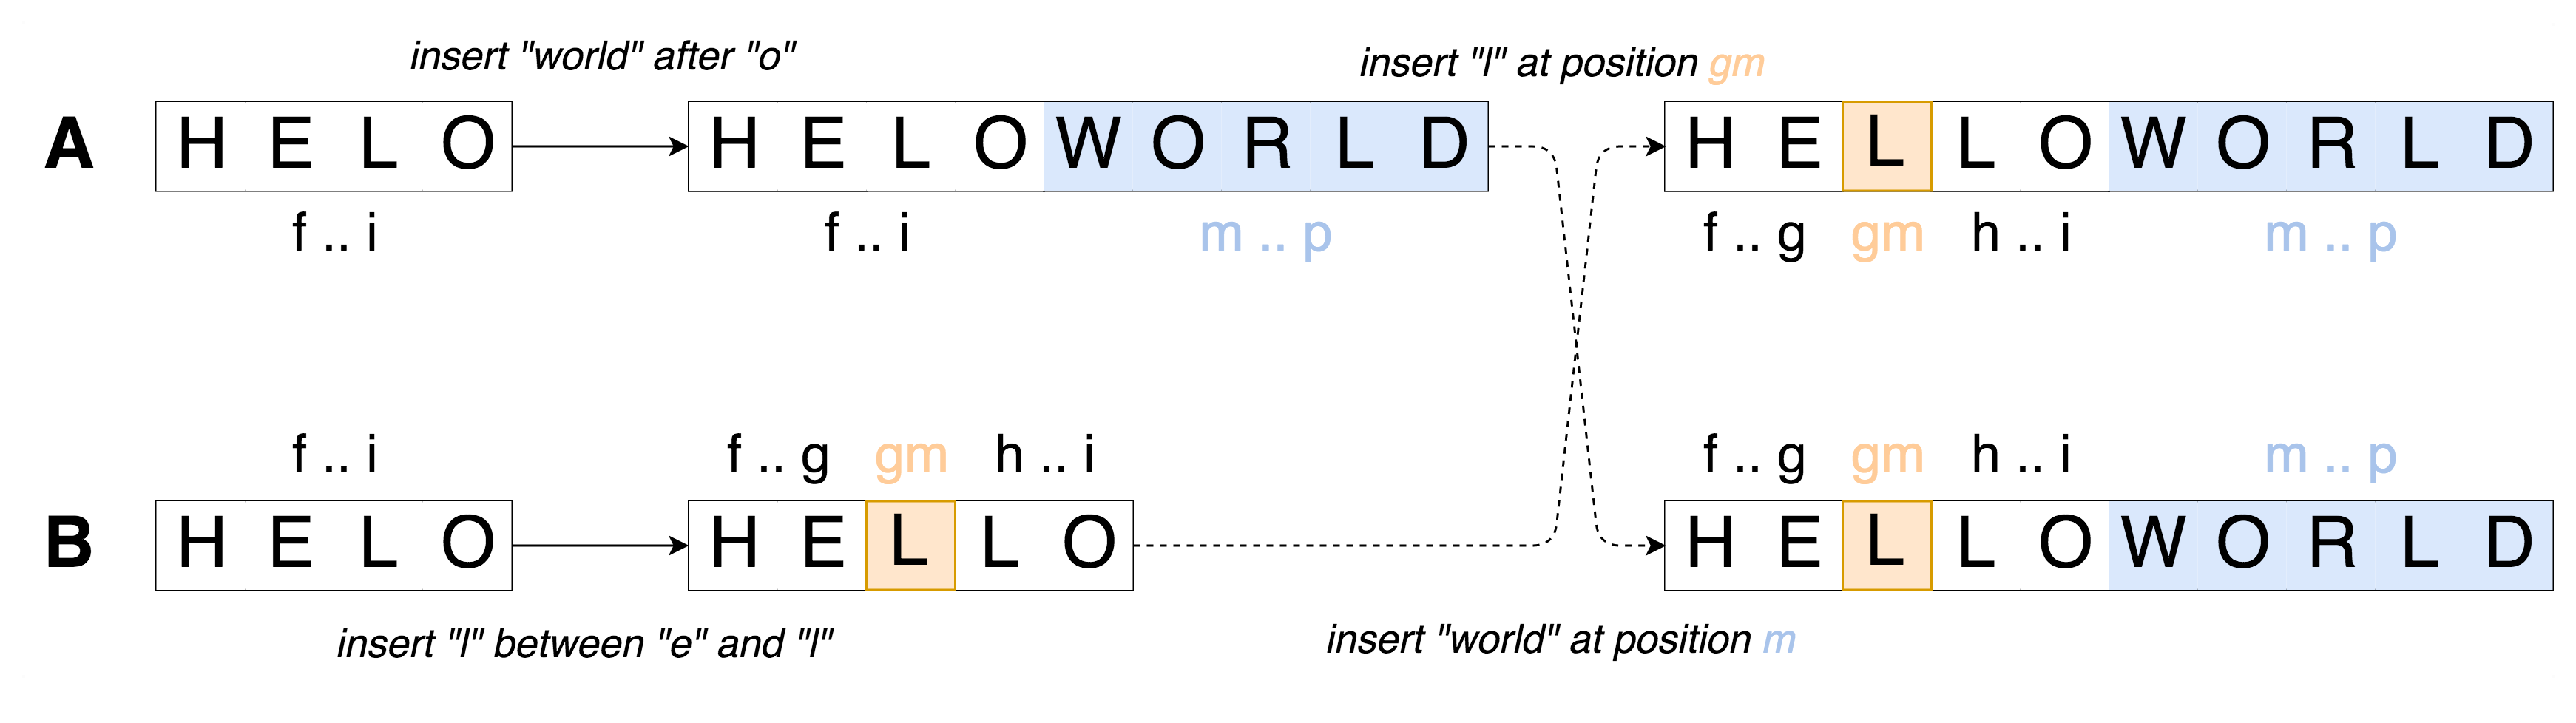
\includegraphics[scale=0.09]{img/final-state.png}<5-5>
    \caption{Example of concurrent $insert$ operations}
  \end{figure}
\end{frame}

\begin{frame}{Declining performances}
  \begin{itemize}
    \item Operations performed may lead to an inefficient internal representation
  \end{itemize}
  \begin{figure}
    
\includegraphics[scale=0.15]{img/worst-case.png}
    \caption{Example of inefficient internal representation}
  \end{figure}
  \begin{itemize}
    \item The more blocks we have:
    \begin{itemize}
      \item The more metadata we store
      \item The longer it takes to browse the sequence to $insert$ or $delete$ an element
    \end{itemize}
  \end{itemize}
\end{frame}

\begin{frame}[standout]
  How to reduce the footprint of the metadata ?
\end{frame}

\begin{frame}{Renaming mechanism}
  \begin{itemize}
    \item Introduce a $rename$ operation
  \end{itemize}
  \begin{figure}
    
\includegraphics[scale=0.11]{img/renaming-0.png}<1-1>
    
\includegraphics[scale=0.11]{img/renaming-1.png}<2-2>
    
\includegraphics[scale=0.11]{img/renaming-2.png}<3-3>
    
\includegraphics[scale=0.11]{img/renaming-3.png}<4-4>
    
\includegraphics[scale=0.11]{img/renaming.png}<5->
    \caption{Example of renaming}
  \end{figure}
  \begin{itemize}
    \item<2-> Generates a new identifier to the first element, based on its previous identifier
    \item<3-> Then generates contiguous identifiers for all following elements
    \item<6-> Each \emph{rename} marks the beginning of a new \emph{epoch}
  \end{itemize}
\end{frame}

\begin{frame}{Handling concurrent operations}
  \begin{itemize}
    \item Others can perform updates concurrently to a \emph{rename} operation
    \item Apply them as such could lead to inconsistencies
  \end{itemize}
  \begin{figure}
    \includegraphics[scale=0.09]{img/concurrent-insert-inconsistency.png}
    \caption{Example of inconsistency}
  \end{figure}
\end{frame}

\begin{frame}{Rewriting concurrent operations}
  \begin{itemize}
    \item Define rewriting rules to transform identifiers from one \emph{epoch} to another
    \item Upon reception of concurrent operations, rewrite identifiers before applying them
  \end{itemize}
  \begin{figure}
    \includegraphics[scale=0.09]{img/concurrent-insert-rewritted.png}
    \caption{Example of rewriting}
  \end{figure}
\end{frame}

\begin{frame}{Handling concurrent \emph{rename}}
  \begin{itemize}
    \item Define a total order between \emph{rename} operations
    \item Pick a "winner" operation between concurrent \emph{renames}
    \item Define additional rewriting rules to \emph{undo} the effect of "losing" ones
  \end{itemize}
\end{frame}

\begin{frame}{Conclusion}
  \begin{itemize}
    \item Propose a fully distributed renaming mechanism for \emph{LogootSplit}
    \item Allows to reinitialize the footprint of the \ac{CRDT} without coordination

    \bigskip

    \item Implemented in MUTE \cite{nicolas:hal-01655438}, our P2P collaborative text editor
  \end{itemize}
\end{frame}

\begin{frame}{Next steps}

  \begin{block}{Provide a formal proof}
    \begin{itemize}
      \item Need to ensure the correctness of our algorithm
    \end{itemize}
  \end{block}

  \medskip

  \begin{block}{Benchmark the mechanism}
    \begin{itemize}
      \item Measure its impact on the performances
      \item Compare different strategies
    \end{itemize}
  \end{block}

  \medskip

  \begin{block}{Generalize the approach to other \acp{CRDT}}
  \end{block}
\end{frame}

\begin{frame}[standout]
  Thanks for your attention, any questions?
  \vspace{3em}
  \begin{center}
    \ccby
  \end{center}
\end{frame}

\begin{frame}[allowframebreaks]
  \frametitle{References}
  \bibliographystyle{abbrv}
  \bibliography{biblio}
\end{frame}

% \begin{frame}{Identifier-based \acp{CRDT}}
%   \begin{block}{Identifiers}
%     \begin{itemize}
%       \item Attached to elements or updates
%       \item Have to comply to several constraints
%       \begin{itemize}
%         \item Unique
%         \item Immutable
%         \item Order relation
%         \item Many others
%       \end{itemize}
%       \item Achieve transaction-less and commutative updates
%     \end{itemize}
%   \end{block}
%   \begin{alertblock}{Limits}<2->
%     \begin{itemize}
%       \item Unbounded size of identifiers
%       % TODO: Soit ils grossissent très vite, soit tombstones
%       \item Efficiency decreasing over time
%     \end{itemize}
%   \end{alertblock}
% \end{frame}

% \begin{frame}{Research problem}
%   \begin{block}{Reduce size of identifiers}
%     \begin{itemize}
%       \item Renaming problem\cite{AlistarhAGG2011}
%     \end{itemize}
%   \end{block}
%   \begin{alertblock}<2->{Make identifiers mutable again}
%     \begin{itemize}
%       \item Trade-off mutability/immutability
%     \end{itemize}
%   \end{alertblock}
% \end{frame}

\end{document}
